% Created 2022-07-29 Fri 18:16
% Intended LaTeX compiler: pdflatex
\documentclass[smaller, aspectratio=1610]{beamer}
\usepackage[utf8]{inputenc}
\usepackage[T1]{fontenc}
\usepackage{graphicx}
\usepackage{longtable}
\usepackage{wrapfig}
\usepackage{rotating}
\usepackage[normalem]{ulem}
\usepackage{amsmath}
\usepackage{amssymb}
\usepackage{capt-of}
\usepackage{hyperref}
\setbeamertemplate{navigation symbols}{}
\usepackage{verbatim, multicol, tabularx}
\usepackage{sourcecodepro}
\usepackage[T1]{fontenc}
\usepackage{amsmath,amsthm, amssymb, latexsym, listings, qtree}
\lstset{extendedchars=\true, inputencoding=utf8, frame=tb, aboveskip=1mm, belowskip=0mm, showstringspaces=false, columns=fixed, basicstyle={\footnotesize\ttfamily}, numbers=left, frame=single, breaklines=true, breakatwhitespace=true, tabsize=4,  keywordstyle=\color{blue}, identifierstyle=\color{violet}, stringstyle=\color{teal}, commentstyle=\color{darkgray}}
\setbeamertemplate{footline}[frame number]
\hypersetup{colorlinks=true,urlcolor=blue,bookmarks=true}
\setlength{\parskip}{.25\baselineskip}
\usetheme{default}
\date{}
\title{Values and Variables}
\hypersetup{
 pdfauthor={},
 pdftitle={Values and Variables},
 pdfkeywords={},
 pdfsubject={},
 pdfcreator={Emacs 28.1 (Org mode 9.5.2)},
 pdflang={English}}
\begin{document}

\maketitle


\section{Values and Variables}
\label{sec:org503209e}

\begin{frame}[label={sec:orgbd0c550}]{Languages and Computation}
Every powerful language has three mechanisms for combining simple ideas to form more complex ideas:(\href{http://mitpress.mit.edu/sicp/full-text/book/book-Z-H-10.html}{SICP 1.1})

\begin{itemize}
\item \alert{primitive expressions}, which represent the simplest entities the language is concerned with,
\item \alert{means of combination}, by which compound elements are built from simpler ones, and
\item \alert{means of abstraction}, by which compound elements can be named and manipulated as units.
\end{itemize}

Today we'll begin learning Python's facilities for primitive expresions, combination, and elementary abstraction.
\end{frame}

\begin{frame}[label={sec:orgcaa7a54}]{Values}
\begin{center}

\includegraphics[height=.7\textheight]{../../images/value-uga-shirt.jpeg}
\end{center}
\end{frame}

\begin{frame}[label={sec:org5172f44},fragile]{Expressions}
 \begin{description}
\item[{value}] a well-defined chunk of data in memory
\item[{expression}] a sequence of symbols that can be \alert{evaluated} to produce a value
\end{description}

When you an expression into the Python REPL, Python evaluates it and prints its value.

\lstset{language=Python,label= ,caption= ,captionpos=b,numbers=none}
\begin{lstlisting}
>>> 1
1
>>> 3.14
3.14
>>> "pie"
'pie'
\end{lstlisting}

The simplest expressions are \alert{literal} values, as in the examples above.

\begin{description}
\item[{literal}] a textual representation of a value in source code.
\end{description}

Compound expressions combine values using operators.  Here the \texttt{+} operator combines the two literal values \texttt{2} and \texttt{3} -- the \alert{operands} -- to produce the value \texttt{5}:

\lstset{language=Python,label= ,caption= ,captionpos=b,numbers=none}
\begin{lstlisting}
>>> 2 + 3
5
\end{lstlisting}

Have a Python REPL session open for this lesson so you can follow along and try your own ideas.
\end{frame}

\begin{frame}[label={sec:orgb79d107},fragile]{Types}
 You can think of a type
\begin{itemize}
\item structurally: as an interpretation of the bits comprising a chunk of data,
\item denotationally: as a set of values, or
\item abstraction-based: as the set of operations available for a type.
\end{itemize}

All values have types. Python can tell you the type of a value with the built-in \texttt{type} function:

\lstset{language=Python,label= ,caption= ,captionpos=b,numbers=none}
\begin{lstlisting}
>>> type(1)
<class 'int'>
>>> type(3.14)
<class 'float'>
>>> type("pie")
<class 'str'>
\end{lstlisting}

\begin{itemize}
\item What's the type of \texttt{'1'}?
\end{itemize}
\end{frame}

\begin{frame}[label={sec:org4fd7bbf},fragile]{Variables}
 Think of variable as a name for a value. You bind a value to a variable using an assignment statement (or by passing an argument to a function), after which the variable \alert{denotes} the value:

\lstset{language=Python,label= ,caption= ,captionpos=b,numbers=none}
\begin{lstlisting}
>>> a = "Ok"
>>> a
'Ok'
\end{lstlisting}

\texttt{=} is the assignment operator.  An assignment statement has the form:

\begin{quote}
\texttt{<variable\_name> = <expression>}
\end{quote}

You can unbind a variable with the \texttt{del} function.

\lstset{language=Python,label= ,caption= ,captionpos=b,numbers=none}
\begin{lstlisting}
>>> del(a)
>>> a
Traceback (most recent call last):
  File "<stdin>", line 1, in <module>
NameError: name 'a' is not defined
\end{lstlisting}

Variable names, or identifiers, may contain letters, numbers, or underscores and may not begin with a number.

\begin{itemize}
\item What happens when you execute this assignment statement?
\end{itemize}

\lstset{language=Python,label= ,caption= ,captionpos=b,numbers=none}
\begin{lstlisting}
>>> 16_candles = "Molly Ringwald"
\end{lstlisting}
\end{frame}

\begin{frame}[label={sec:org622cf5e},fragile]{Keywords}
 Python reserves some identifiers for its own use.

\lstset{language=Python,label= ,caption= ,captionpos=b,numbers=none}
\begin{lstlisting}
False      class      finally    is         return
None       continue   for        lambda     try
True       def        from       nonlocal   while
and        del        global     not        with
as         elif       if         or         yield
assert     else       import     pass
break      except     in         raise
\end{lstlisting}


\begin{itemize}
\item What happens when you execute this assignment statement?
\end{itemize}

\lstset{language=Python,label= ,caption= ,captionpos=b,numbers=none}
\begin{lstlisting}
>>> class = "CS 2316"
\end{lstlisting}


\begin{itemize}
\item What happens if you use \texttt{print} as a variable name?
\item How can you fix it?
\end{itemize}
\end{frame}

\begin{frame}[label={sec:org4fcd87e},fragile]{Assignment Semantics}
 \texttt{=} stores the memory address of the value on the right-hand side in a memory cell referenced by the variable on the left hand side.  Python variables refer to these pointer memory cells. Evaluate these assignment statements in a Python REPL and make sure you understand them.

\begin{columns}
\begin{column}{0.3\columnwidth}
\begin{block}{}
\lstset{language=Python,label= ,caption= ,captionpos=b,numbers=none}
\begin{lstlisting}
a = 1
b = 2
\end{lstlisting}

\begin{center}
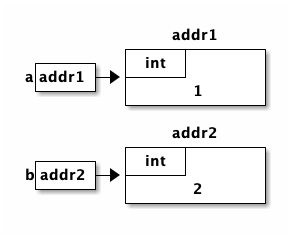
\includegraphics[width=1.75in]{diagrams/assignment-semantics1.png}
\end{center}
\end{block}
\end{column}

\begin{column}{0.3\columnwidth}
\begin{block}{}
\lstset{language=Python,label= ,caption= ,captionpos=b,numbers=none}
\begin{lstlisting}
a = b
\end{lstlisting}

\begin{center}
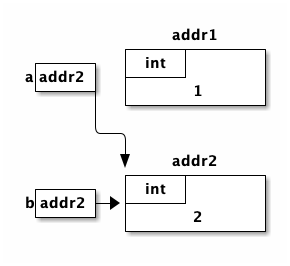
\includegraphics[width=1.75in]{diagrams/assignment-semantics2.png}
\end{center}
\end{block}
\end{column}

\begin{column}{0.3\columnwidth}
\begin{block}{}
\lstset{language=Python,label= ,caption= ,captionpos=b,numbers=none}
\begin{lstlisting}
b = 42
\end{lstlisting}

\begin{center}
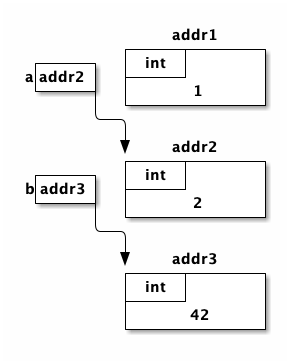
\includegraphics[width=1.75in]{diagrams/assignment-semantics3.png}
\end{center}
\end{block}
\end{column}
\end{columns}
\end{frame}

\begin{frame}[label={sec:org5cfc232},fragile]{Types as Interpretations of Bits}
 You can represent the byte \texttt{01000001} with \texttt{b'\textbackslash{}x41'}.  \texttt{\textbackslash{}x} means the characters that follow are hexadecimal digits. You will probably never do this sort of thing in Python.  These examples simply illustrate what we mean by viewing types as interpretations of bits.


\begin{columns}
\begin{column}{0.55\columnwidth}
\begin{block}{}
If you interpret those bits as an \texttt{int} you get:

\lstset{language=Python,label= ,caption= ,captionpos=b,numbers=none,basicstyle=\ttfamily\scriptsize}
\begin{lstlisting}
>>> n = int.from_bytes(b'\x41', byteorder='little')
>>> n
65
\end{lstlisting}

\begin{center}
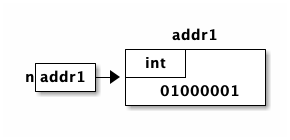
\includegraphics[width=1.75in]{diagrams/type-bits-int.png}
\end{center}
\end{block}
\end{column}

\begin{column}{0.45\columnwidth}
\begin{block}{}
If you interpret the same bits as a \texttt{str}:

\lstset{language=Python,label= ,caption= ,captionpos=b,numbers=none,basicstyle=\ttfamily\scriptsize}
\begin{lstlisting}
>>> s = str(b'\x41', encoding='utf-8')
>>> s
'A'
\end{lstlisting}

\begin{center}
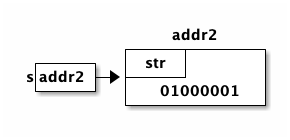
\includegraphics[width=1.75in]{diagrams/type-bits-str.png}
\end{center}
\end{block}
\end{column}
\end{columns}
\end{frame}


\begin{frame}[label={sec:org26235da},fragile]{Types as Sets of Values}
 \begin{itemize}
\item \texttt{int} is like the set of integers, \(\mathbb{Z}\).
\item \texttt{float} is like the set of real numbers, \(\mathbb{R}\).
\item \texttt{bool} is the finite set of values \texttt{True} and \texttt{False}.
\item \texttt{str} is the set of all sequences of characters from the UTF-8 character set.
\end{itemize}

Again, this is not terribly useful in Python unless you want to think of compound expressions in set theoretic terms.
\end{frame}

\begin{frame}[label={sec:org4a7bb93},fragile]{Aside: The Sizes of Types}
 One of the convenient things about Python is that you don't have to worry about overflow or underflow\footnote{In regular Python you don't have to worry about type size limits, but in scientific Python, which relies on libraries written in C, C++ and Fortran you do.}. For example, as in mathematics, the set \texttt{int} is unbounded:

\lstset{language=Python,label= ,caption= ,captionpos=b,numbers=none}
\begin{lstlisting}
>>> import sys
>>> x = sys.maxsize
>>> x
9223372036854775807 # That's ~ 9.2 quintillion, i.e., 9.2e+18
>>> x = x + 1
>>> x
9223372036854775808
>>>
\end{lstlisting}

But you should consider \texttt{sys.maxsize}, the word size of your processor (64 bits in this example, since \texttt{sys.maxsize} \(= 2^{63} - 1\)), to be the practical limit, because it's the theoretical limit \footnote{Not strictly true, but practically true.} of addressable RAM and thus the largest possible (but certainly impractical) array you could store in main memory and therefore, as you'll learn later, the largest possible list index.
\end{frame}

\begin{frame}[label={sec:org00def15},fragile]{Types as Sets of Operations}
 Types determine which operations are available on values. For example, exponentiation is defined for numbers (like int or float):


\lstset{language=Python,label= ,caption= ,captionpos=b,numbers=none}
\begin{lstlisting}
>>> 2**3
8
\end{lstlisting}


\ldots{} but not for \texttt{str} (string) values:


\lstset{language=Python,label= ,caption= ,captionpos=b,numbers=none}
\begin{lstlisting}
>>> "pie"**3
Traceback (most recent call last):
  File "<stdin>", line 1, in <module>
TypeError: unsupported operand type(s) for ** or pow(): 'str' and 'int'
\end{lstlisting}


This is the primary way to think about types in Python.
\end{frame}

\begin{frame}[label={sec:org451c003},fragile]{Overloaded Operators}
 Some operators are overloaded, meaning they have different meanings when applied to different types. For example, + means addition for numbers and concatenation for strings:

\lstset{language=Python,label= ,caption= ,captionpos=b,numbers=none}
\begin{lstlisting}
>>> 2 + 2
4
>>> "Yo" + "lo!"
'Yolo!'
\end{lstlisting}

\texttt{*} means multiplication for numbers and repetition for strings:

\lstset{language=Python,label= ,caption= ,captionpos=b,numbers=none}
\begin{lstlisting}
>>> 2 * 3
6
>>> "Yo" * 3
'YoYoYo'
>>> 3 * "Yo"
'YoYoYo'
\end{lstlisting}
\end{frame}

\begin{frame}[label={sec:org10237e4},fragile]{Expression Evaluation}
 Mathematical expressions are evaluated using precedence and associativity rules as you would expect from math:

\lstset{language=Python,label= ,caption= ,captionpos=b,numbers=none}
\begin{lstlisting}
>>> 2 + 4 * 10
42
\end{lstlisting}

If you want a different order of operations, use parentheses:

\lstset{language=Python,label= ,caption= ,captionpos=b,numbers=none}
\begin{lstlisting}
>>> (2 + 4) * 10
60

\end{lstlisting}

Note that precedence and associativity rules apply to overloaded versions of operators as well:

\lstset{language=Python,label= ,caption= ,captionpos=b,numbers=none}
\begin{lstlisting}
>>> "Honey" + "Boo" * 2
'HoneyBooBoo'
\end{lstlisting}

\begin{itemize}
\item How could we modify the expression above to evaluate to 'HoneyBooHoneyBoo' ?
\end{itemize}
\end{frame}

\begin{frame}[label={sec:orge48332b},fragile]{Python is Dynamically Typed}
 Python is dynamically typed, meaning that types are not resoved until run-time. This means two things practically:

\begin{enumerate}
\item Values have types, variables don't:
\lstset{language=Python,label= ,caption= ,captionpos=b,numbers=none}
\begin{lstlisting}
   >> a = 1
   >>> type(a)
   <class 'int'>
   >>> a = 1.1 # would be disallowed in a statically typed language
   >>> type(a)
   <class 'float'>
\end{lstlisting}
\item Python doesn't report type errors until run-time. We'll see many examples of this fact.
\end{enumerate}

Evaluate the following expressions in the Python REPL.  Be sure to type them exactly as written.

\begin{itemize}
\item \texttt{2 + 3}
\item \texttt{'2' + '3'}
\item \texttt{'2' + 3}
\item \texttt{2 + '3'}
\end{itemize}
\end{frame}

\begin{frame}[label={sec:org9f38750},fragile]{Type Conversions}
 Convert a value to a different type by applying conversions named after the target type.

\lstset{language=Python,label= ,caption= ,captionpos=b,numbers=none}
\begin{lstlisting}
>>> int(2.9)
2
>>> float(True)
1.0
>>> int(False)
0
>>> str(True)
'True'
>>> int("False")
Traceback (most recent call last):
  File "<stdin>", line 1, in <module>
ValueError: invalid literal for int() with base 10: 'False'
\end{lstlisting}

Modify the following expressions to produce the indicated results.

\begin{itemize}
\item \texttt{'2' + 3} (we want \texttt{'23'})
\item \texttt{2 + '3'} (we want \texttt{5})
\end{itemize}
\end{frame}

\begin{frame}[label={sec:orga5be55d},fragile]{Assignment Semantics}
 Python evaluates the expression on the right-hand side, then binds the expression's value to the variable on the left-hand side. Variables can be reassigned:

\lstset{language=Python,label= ,caption= ,captionpos=b,numbers=none}
\begin{lstlisting}
>>> a = 'Littering and ... '
>>> a
'Littering and ... '
>>> a = a * 2
>>> a
'Littering and ... Littering and ... '
>>> a = a * 2
>>> a              # I'm freakin' out, man!
'Littering and ... Littering and ... Littering and ... Littering and ... '
\end{lstlisting}

Note that the value of \texttt{a} used in the expression on the right hand side is the value it had before the assignment statement.

What's the type of \texttt{a}?
\end{frame}

\begin{frame}[label={sec:orga7979b0}]{Boolean Values}
There are 10 kinds of people:

\begin{itemize}
\item those who know binary, and
\item those who don't.
\end{itemize}
\end{frame}

\begin{frame}[label={sec:org29723e7},fragile]{Python Booleans}
 In Python, boolean values have the \texttt{bool} type. Four kinds of boolean
expressions:

\begin{itemize}
\item \texttt{bool} literals: \texttt{True} and \texttt{False}
\item \texttt{bool} variables
\item expressions formed by combining non-\texttt{bool} expressions with comparison operators
\item expressions formed by combining \texttt{bool} expressions with logical operators
\end{itemize}
\end{frame}

\begin{frame}[label={sec:orgd43edae},fragile]{Boolean Expressions}
 \begin{block}{Comparison operators:}
\begin{itemize}
\item Equal to: \texttt{==}, like \(=\) in math

\begin{itemize}
\item Remember, \texttt{=} is assignment operator, \texttt{==} is comparison operator!
\end{itemize}

\item Not equal to: \texttt{!=}, like \(\ne\) in math
\item Greater than: \texttt{>}, like \(>\) in math
\item Greater than or equal to: \texttt{>=}, like \(\ge\) in math
\end{itemize}

\lstset{language=Python,label= ,caption= ,captionpos=b,numbers=none}
\begin{lstlisting}
1 == 1 # True
1 != 1 # False
1 >= 1 # True
1 > 1  # False
\end{lstlisting}
\end{block}

\begin{block}{Logical operators:}
\lstset{language=Python,label= ,caption= ,captionpos=b,numbers=none}
\begin{lstlisting}
True and True  # True
True and False # False
True or False  # True
False or False # False
not True       # False
\end{lstlisting}


\begin{itemize}
\item What is the value of \texttt{"foo" == "Foo"}?
\item What is the value of \texttt{"foo" > "Foo"}?
\end{itemize}
\end{block}
\end{frame}

\begin{frame}[label={sec:org6cf4460},fragile]{Truth in Python}
 The zero values of built-in types are equivalent to \texttt{False}:

\begin{itemize}
\item boolean \texttt{False}
\item \texttt{None}
\item integer \texttt{0}
\item float \texttt{0.0}
\item empty string \texttt{""}
\item empty list \texttt{[]}
\item empty tuple \texttt{()}
\item empty dict \texttt{\{\}}
\item empty set \texttt{set()}
\end{itemize}

All other values are equivalent to True.

\begin{itemize}
\item Every value in Python is either \alert{truthy} or \alert{falsey} and can be used in a boolean context.
\end{itemize}
\end{frame}

\begin{frame}[label={sec:orgc49aeed},fragile]{Short-circuit Evaluation}
 Logical expressions use short-circuit evaluation:

\begin{itemize}
\item \texttt{or} only evaluates second operand if first operand is \texttt{False}
\item \texttt{and} only evaluates second operand if first operand is \texttt{True}
\end{itemize}

What are the values of the following expressions?

\begin{itemize}
\item \texttt{True and False}
\item \texttt{True and 0}
\item \texttt{True and []}
\item \texttt{True and None}
\item \texttt{type(True and None)}
\item \texttt{False or 1}
\item \texttt{True or 1}
\item \texttt{1 and "done"}
\item \texttt{1 == 1 or 0}
\item \texttt{1 == 1 and 0}
\item \texttt{1 == (1 and 0)}
\end{itemize}


Guard idiom: \texttt{(b == 0) or print(a / b)}, or \texttt{(b != 0) and print(a / b)}
\end{frame}

\begin{frame}[label={sec:orgefc792b}]{Values, Variables, and Expression}
\begin{itemize}
\item Values are the atoms of computer programs
\item Expressions produce values
\item We combine values using operators and functions to form compound expressions
\item Variables are identifiers that denote values
\begin{itemize}
\item Identifiers also denote functions, classes, modules and packages
\end{itemize}
\item Choose identifiers carefully to create beautiful, readable programs
\end{itemize}
\end{frame}
\end{document}